\section{Path}

The class Path represents the road that the mobs walk along. Each track has a unique path. Path has a list of the coordinates for the checkpoints of the road. A checkpoint is a point where the direction of the path changes. 

The Path in itself is not visible to the user, but the background image of the track contains a visual representation of it. The path is used by two classes. Firstly, the mobs use it when they update their position on the map. They use the coordinates to calcuate in which direction they should move. Secondly, GameView uses Path to calculate where the user can place towers, since the user is not allowed to place towers on the path.

The Path class is implemented as a singleton, meaning that only one object of the class can exist. When the track is changed, the Path object is reset and reused. The Path object is, just like the MobFactory object, first initialized when the player chooses a track from the progression map. The Path and MobFactory singletons are almost identical in their structure, but they handle different kinds of data.

When the path is initialized information is read from an XML-file called initpaths, which is structured as a string array, where every item is a checkpoint. Figure ~\ref{fig:codeExInitPathXML} shows the structure of initpath.

%-----
%- Code snippet initpath.xml
%-----
\begin{figure}[htb]

\begin{small}
\verbatiminput{code/initpathXML.java}
\end{small}

\caption{Caption}
\label{fig:codeExInitPathXML}

\end{figure}
%-----

The initiation of Path is structured in a similar way as MobFactory. It contains two nested loops to iterate over every \begin{math} <array> \end{math} tag which represents a track and every \begin{math} <item> \end{math} tag which contains coordinates for the checkpoints. The data is also saved in an ArrayList, where every element contains an ArrayList of coordinates.

%----
%- Image datastructure path
%----
\begin{figure}[here]

\begin{center}
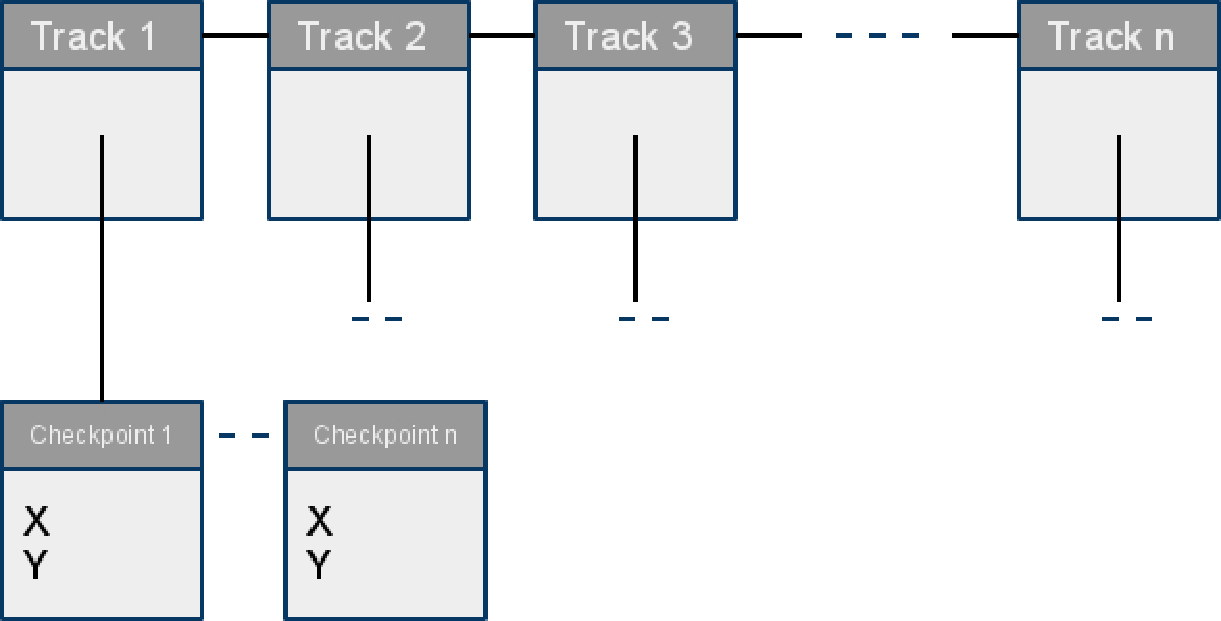
\includegraphics[scale=0.5]{pics/chapters/chapter4/pathlist2}
\end{center}

\caption{Caption}
\label{fig:dataStructurePath}
\end{figure}
%----
